\documentclass{beamer}[10pt]
\usepackage[utf8]{inputenc}
\usepackage{tikz}
\usetikzlibrary{ shapes, arrows, positioning}
\usepackage{amsmath}
\usepackage{tabularx}
\usepackage{hyperref}
\usetheme{Warsaw}
\usefonttheme{serif}



\tikzstyle{boxes} = [rectangle, minimum width=3 cm , minimum height = 1 cm, text centered , draw=black, fill=orange!30]





\title{\textrm{Assignment-2}}
\subtitle{\textrm{Software Systems Lab}}
\author{\textit{Hrishikesh Pable }}
\institute{IIT Dharwad \\
\href{https://www.iitdh.ac.in/}{\texttt{https://www.iitdh.ac.in/}}}
\date{August 11, 2021}

\titlegraphic{
  
\includegraphics[width=3 cm]{Image 2.jpeg}
 }



\begin{document}


\maketitle
%\begin{titlepage}



%\begin{figure}[H]
%    \centering
%    
\includegraphics[scale=0.10]{Image 2.jpeg}
%    \label{fig:fig1}
%\end{figure}

%\end{titlepage}

%\begin{frame}{Sample Frame Title}
%This is some text in the first frame of this latex presentation which is a part of %an assignment given to us under the ssl laboratory course.
    
%\end{frame}

\begin{frame}{Dynamic Programming}
\begin{itemize}
    \item Characteristics of Dynamic Programming
    \begin{enumerate}
        \item \textit{Overlapping Sub-problems}
        \begin{block}{1}
            Subproblems are smaller versions of the original problem. Any problem has overlapping sub-problems if finding its solution involves solving the same subproblem multiple times.
        \end{block}
        \item \textit{Optimal Substructure}
        \begin{block}{2}
            Any problem has optimal substructure property if its overall optimal solution can be constructed from the optimal solutions of its subproblems.
        \end{block}
    \end{enumerate}
\end{itemize}
    
\end{frame}

\begin{frame}{DP Methods}

\begin{itemize}
    \item \textbf{Top-down with Memoization}
    \begin{block}{1}
    In this approach, we try to solve the bigger problem by recursively finding the solution to smaller sub-problems. Whenever we solve a sub-problem, we cache its result so that we don’t end up solving it repeatedly if it’s called multiple times. Instead, we can just return the saved result.

    \end{block}
    
    \item <2-> \textbf{Bottom-up with Tabulation}
    \begin{alertblock}{2}
    Tabulation is the opposite of the top-down approach and avoids recursion. In this approach, we solve the problem “bottom-up” (i.e. by solving all the related sub-problems first).

    
    \end{alertblock}
\end{itemize}
    
\end{frame}

\begin{frame}{Algorithms}

\transdissolve

\label{Algorithms}
\setbeamercovered{transparent}
\begin{itemize}
    \item Divide and conquer \pause
    \invisible \item Greedy Algorithm \pause
    \invisible \item Dynamic Programming 
\end{itemize}
    
\end{frame}

\begin{frame}{Divide and Conquer}
\only<1>
{Example:\\
\textbf{Quick-Sort:The average case run time of quick sort is} $O(n*\log n)$\textbf{.This case happens when we don't exactly \\ get evenly balanced partitions.}}

\only<2>
{\textcolor{red}{Example:} \\
Merge-Sort:\textcolor{orange}{The time complexity of Merge Sort is $O(n*\log n)$.Merge Sort is useful for sorting linked lists in $O(n*\log n)$ time.}}
    
\end{frame}

\begin{frame}{Hyperlinks}
\begin{itemize}
    \item Divide and Conquer
    \item \hyperlink{Algorithms}{\beamergotobutton{Greedy Algorithm}}
    \item \hyperlink{Algorithms}{\beamergotobutton{Dynamic Programming}}
\end{itemize}
    
\end{frame}


\begin{frame}{List of Data Structures}
\setbeamersize{descriptionwidth=0.65cm}
\setbeamercovered{transparent}
    \begin{itemize}
        \item Primitive \pause
        \item Non-Primitive \pause  \newline \\
        \onslide<3->
        \begin{itemize}
            \item \textit{Linear}
            \begin{description}
                \item[$\bullet$]<4-> \textbf{Static}
                \begin{enumerate}
                    \item<5-> Array \newline
                \end{enumerate}
                \item[$\bullet$]<4-> \textbf{Dynamic}
                \begin{enumerate}
                    \item<5-> Linked List
                    \item<5-> Stack
                    \item<5-> Queue \newline
                \end{enumerate}
            \end{description}
            \onslide<6->
            \item \textit{Non-Linear}
            \begin{enumerate}
                \item<6-> Tree
                \item<6-> Graph
            \end{enumerate}
        \end{itemize}
    \end{itemize}
\end{frame}
\begin{frame}{Data Structures}

%\begin{tikzpicture}
%    \node (ds) [boxes] {Data Structure}
%    \node (pds) [boxes, below of=ds, xshift=2 cm, %yshift=2 cm] {Non-Primitive Data Structures}
%\end{tikzpicture}
    
\begin{figure}
    \centering
    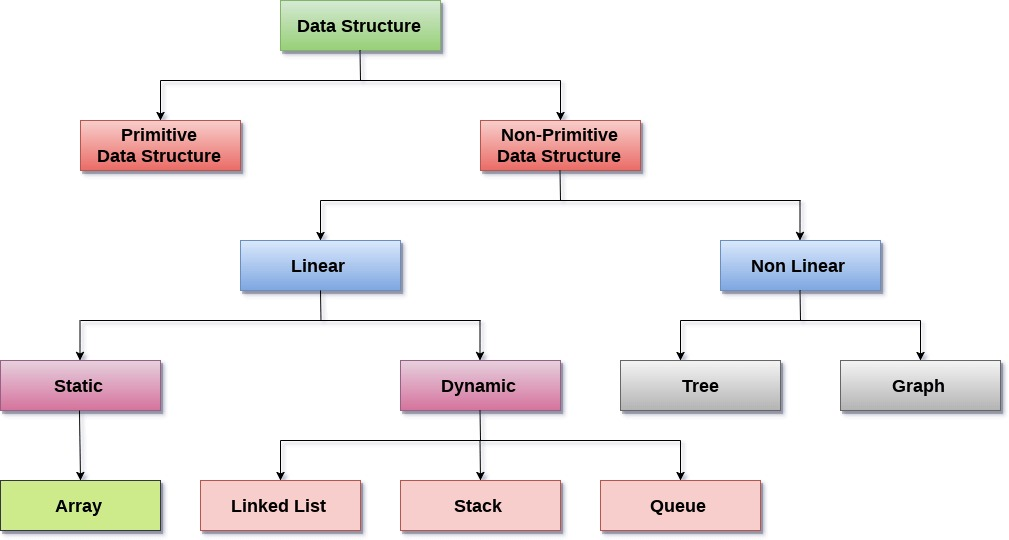
\includegraphics[scale=0.25]{Image 1.jpeg}
    \caption{1}
    \label{fig:my_label}
\end{figure}
    
\end{frame}

\begin{frame}{}
    
    \begin{center}
        \begin{table}[t]
            \centering
            \begin{tabular}{|c|c|c|c|}
            \hline
            Algorithm  & Best Case  & Average Case & Worst Case  \\
             \hline
             \hline
             Linear Search & $O(1)$ & $O(n)$ & $O(n)$ \\
             Binary Search & $O(1)$ & $O(\log n)$ & $O(\log n)$ \\
             Bubble sort & $O(n)$ & $O(n^2)$ & $O(n^2)$ \\
             Selection sort & $O(n^2)$ & $O(n^2)$ & $O(n^2)$ \\
             \hline
            \end{tabular}
            \caption{1}
            \label{tab:table1}
        \end{table}
    \end{center}
    
    \begin{theorem} [Trigonometric Identity]
    $Sin ^2 \theta + Cos ^2 \theta = 1$
    \end{theorem}
    
\transboxin    

\end{frame}

\begin{frame}
\begin{theorem}
\textit{Let a, b, c be lengths of right angle triangle.}\\
\textbf{\textit{By definition}}

$$sin\theta = b/c\left(\frac{oppositeside}{hypotenuse}\right)$$

$$cos\theta = a/c\left(\frac{adjacentside}{hypotenuse}\right)$$

$sin^2\theta + cos^2\theta = \frac{b^2}{c^2} + \frac{a^2}{c^2} = \frac{a^2+b^2}{c^2} $ \\
\bigskip
\textbf{\textit{From Pythagorus theorem}} \\
\bigskip
$c^2 = a^2 + b^2$ \\
\bigskip
$\frac{a^2+b^2}{c^2} = 1$ $\Longrightarrow$ $sin^2\theta + cos^2\theta = 1$ \\
\bigskip
\textbf{\textit{Hence Proved.}}
    
\end{theorem}

\end{frame}

\begin{frame}{Multi-line equations}
\transblindshorizontal
\begin{align*}
    f(x) = x^6 + 7x^3y + 50x^3y^2 & + 12x^2y^4 \\
                                  &- 19x^5y^4 - 10x^7y^6 + 7y^4 - m^3n^3
\end{align*}


\begin{align*}
\rho \Delta x \Delta y \Delta z \Delta \tau \partial_t c_i(t,x,\tau) 
& = \rho \Delta x \Delta y \Delta z \Delta \tau (p_i-d_i)  \\
& - \rho \Delta y, \Delta z \Delta \tau [q_{i,x}(t,x+\Delta x/2, y, z, \tau)\\
& \qquad - q_{i,x}(t,x - \Delta x/2, y, z, \tau)]\\
& - \rho \Delta x, \Delta z \Delta  \tau [q_{i,y}(t,x,y+\Delta y/2, y, z, \tau)\\
& \qquad - q_{i,y}(t,x,y - \Delta y/2, z, z, \tau)]\\
& - \rho \Delta x \Delta y \Delta \tau[q_{i,z}(t,x,y,z+\Delta z/2, \tau) \\
& \qquad - q_{i,z}(t,x,y,z-\Delta z/2, \tau)]
\end{align*}
\end{frame}





\end{document}
